\documentclass[usenames,dvipsnames,tikz]{standalone}
\usetikzlibrary{shapes.geometric}
\usepackage{xcolor}
\colorlet{myBlue}{RoyalBlue!35!Cerulean}
\colorlet{myRed}{Red!85!YellowOrange}
\usepackage{tikz}
\usepackage{standalone}
\begin{document}
	
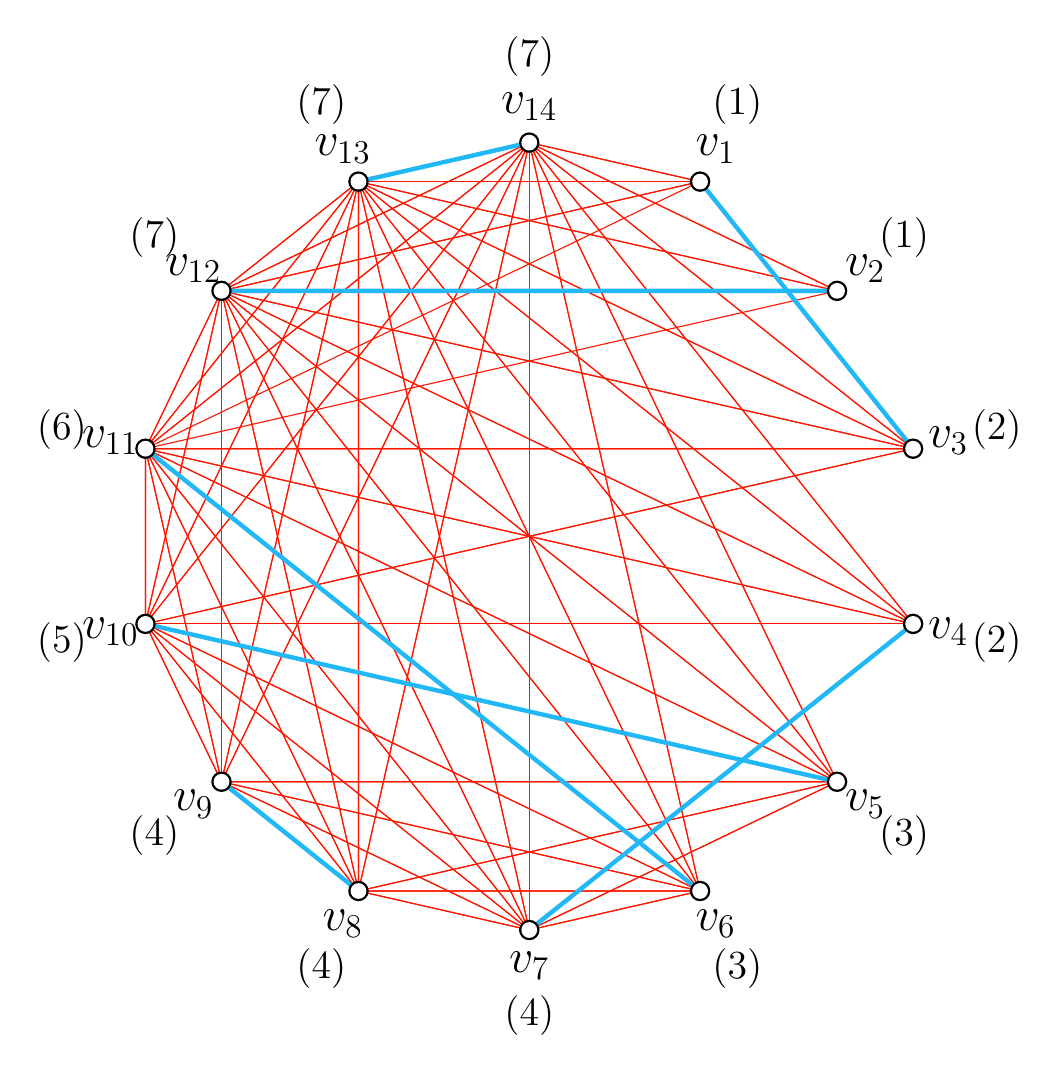
\begin{tikzpicture}
%Values of nodes:
% 0 = 1
% 1 = 1
% 2 = 2
% 3 = 2
% 4 = 3
% 5 = 3
% 6 = 4
% 7 = 4
% 8 = 4
% 9 = 5
% 10 = 6
% 11 = 7
% 12 = 7
% 13 = 7
% threshold tau = 7

\foreach \n/\value in {1/1, 2/1, 3/2, 4/2, 5/3, 6/3, 7/4, 8/4, 9/4, 10/5, 11/6, 12/7, 13/7, 14/7}
	\fill (90-\n*25.71428571:5cm) coordinate (v\n) circle [radius = 0.1]
		++(90-\n*25.71428571:13pt) node {\LARGE{$v_{\n}$}}
		++(90-\n*25.71428571:18pt) node {\Large{(\value)}};
\foreach \m/\n in {1/12,1/13,1/14,2/13,2/14,3/10,3/11,3/12,3/13,3/14,4/10,4/11,4/12,4/13,4/14,5/7,5/8,5/9,5/11,5/12,5/13,5/14,6/7,6/8,6/9,6/10,6/12,6/13,6/14,7/5,7/6,7/8,7/9,7/10,7/11,7/12,7/13,7/14,8/5,8/6,8/7,8/10,8/11,8/12,8/13,8/14,9/5,9/6,9/7,9/10,9/11,9/12,9/13,9/14,10/3,10/4,10/6,10/7,10/8,10/9,10/11,10/12,10/13,10/14,11/1,11/2,11/3,11/4,11/5,11/7,11/8,11/9,11/10,11/12,11/13,11/14,12/1,12/3,12/4,12/5,12/6,12/7,12/8,12/9,12/10,12/11,12/13,12/14,13/1,13/2,13/3,13/4,13/5,13/6,13/7,13/8,13/9,13/10,13/11,13/12,14/1,14/2,14/3,14/4,14/5,14/6,14/7,14/8,14/9,14/10,14/11,14/12}
	\draw [myRed] (v\n) -- (v\m);
\foreach \m/\n in {1/3, 2/12, 4/7, 5/10, 6/11, 8/9, 13/14}
	\draw [ultra thick, myBlue] (v\n) -- (v\m);
\foreach \n in {1,...,14}
	\fill (90-\n*25.71428571:5cm) coordinate (v\n) circle [radius = 0.13];
\foreach \n in {1,...,14}
	\fill [white] (90-\n*25.71428571:5cm) coordinate (v\n) circle [radius = 0.1];

\end{tikzpicture}
	
\end{document}